\documentclass[10pt]{beamer}\usepackage[]{graphicx}\usepackage[]{color}
% maxwidth is the original width if it is less than linewidth
% otherwise use linewidth (to make sure the graphics do not exceed the margin)
\makeatletter
\def\maxwidth{ %
  \ifdim\Gin@nat@width>\linewidth
    \linewidth
  \else
    \Gin@nat@width
  \fi
}
\makeatother

\definecolor{fgcolor}{rgb}{0.345, 0.345, 0.345}
\newcommand{\hlnum}[1]{\textcolor[rgb]{0.686,0.059,0.569}{#1}}%
\newcommand{\hlstr}[1]{\textcolor[rgb]{0.192,0.494,0.8}{#1}}%
\newcommand{\hlcom}[1]{\textcolor[rgb]{0.678,0.584,0.686}{\textit{#1}}}%
\newcommand{\hlopt}[1]{\textcolor[rgb]{0,0,0}{#1}}%
\newcommand{\hlstd}[1]{\textcolor[rgb]{0.345,0.345,0.345}{#1}}%
\newcommand{\hlkwa}[1]{\textcolor[rgb]{0.161,0.373,0.58}{\textbf{#1}}}%
\newcommand{\hlkwb}[1]{\textcolor[rgb]{0.69,0.353,0.396}{#1}}%
\newcommand{\hlkwc}[1]{\textcolor[rgb]{0.333,0.667,0.333}{#1}}%
\newcommand{\hlkwd}[1]{\textcolor[rgb]{0.737,0.353,0.396}{\textbf{#1}}}%
\let\hlipl\hlkwb

\usepackage{framed}
\makeatletter
\newenvironment{kframe}{%
 \def\at@end@of@kframe{}%
 \ifinner\ifhmode%
  \def\at@end@of@kframe{\end{minipage}}%
  \begin{minipage}{\columnwidth}%
 \fi\fi%
 \def\FrameCommand##1{\hskip\@totalleftmargin \hskip-\fboxsep
 \colorbox{shadecolor}{##1}\hskip-\fboxsep
     % There is no \\@totalrightmargin, so:
     \hskip-\linewidth \hskip-\@totalleftmargin \hskip\columnwidth}%
 \MakeFramed {\advance\hsize-\width
   \@totalleftmargin\z@ \linewidth\hsize
   \@setminipage}}%
 {\par\unskip\endMakeFramed%
 \at@end@of@kframe}
\makeatother

\definecolor{shadecolor}{rgb}{.97, .97, .97}
\definecolor{messagecolor}{rgb}{0, 0, 0}
\definecolor{warningcolor}{rgb}{1, 0, 1}
\definecolor{errorcolor}{rgb}{1, 0, 0}
\newenvironment{knitrout}{}{} % an empty environment to be redefined in TeX

\usepackage{alltt}


%\input{slides_header.tex}
\usepackage{graphicx}
\usepackage{hyperref, url}
\hypersetup{colorlinks,citecolor=myorange,filecolor=red,linkcolor=brown,urlcolor=blue}

\usepackage{longtable,booktabs}
\usepackage{amssymb,amsmath}
\usepackage{animate}
\usepackage{subfig}
\usepackage{tikz}
\usetikzlibrary{shapes.geometric, arrows,shapes.symbols,decorations.pathreplacing}
\tikzstyle{startstop} = [rectangle, rounded corners, minimum width=3cm, minimum height=1cm, draw=black, fill=pinkish,text width=3.5cm]
\tikzstyle{startstop2} = [rectangle, rounded corners, minimum width=3cm, minimum height=1cm, draw=black, fill=background,text width=4.5cm]
\tikzstyle{startstop3} = [rectangle, rounded corners, minimum width=3cm, minimum height=1cm, draw=black, fill=beige,text width=3.0cm]
\tikzstyle{startstop4} = [rectangle, rounded corners, minimum width=3cm, minimum height=1cm, draw=black, fill=pinkish,text width=4.5cm]
\tikzstyle{io} = [trapezium, trapezium left angle=70, trapezium right angle=110, minimum width=2cm, minimum height=1cm, text centered, draw=black, fill=blue!30,text width=1.5cm]
\tikzstyle{process} = [rectangle, minimum width=1cm, minimum height=1cm, text centered, draw=black, fill=orange!30,text width=2cm]
\tikzstyle{decision} = [diamond, minimum width=2cm, minimum height=1cm, text centered, draw=black, fill=green!30]
\tikzstyle{arrow} = [thick,->,>=stealth]
\tikzstyle{both} = [thick,<->,>=stealth, red]


% used for tree of stats tests in 001-introduction
\tikzstyle{startstopstats} = [rectangle, rounded corners, minimum width=2cm, minimum height=.5cm,text centered, draw=black, fill=red!30]
\tikzstyle{iostats} = [trapezium, trapezium left angle=70, trapezium right angle=110, minimum width=2cm, minimum height=.5cm, text centered, draw=black, fill=blue!30]
\tikzstyle{processstats} = [rectangle, minimum width=1.5cm, minimum height=.5cm, text centered, draw=black, fill=orange!30]
\tikzstyle{processbigstats} = [rectangle, minimum width=1.5cm, minimum height=.5cm, text centered, draw=black, fill=orange!30,text width=1.6cm]
\tikzstyle{decisionstats} = [rectangle, minimum width=1cm, minimum height=1cm, text centered, draw=black, fill=green!30,text width=1.6cm]
\tikzstyle{decisionbigstats} = [rectangle, minimum width=1cm, minimum height=1cm, text centered, draw=black, fill=yellow!30,text width=2cm]

\usepackage{pifont}% http://ctan.org/pkg/pifont
\newcommand{\cmark}{\ding{51}}%
\newcommand{\xmark}{\ding{55}}%

\usepackage{ulem} % for strikeout

\usepackage{xcolor}
\usepackage{color, colortbl}
\definecolor{lightgray}{RGB}{200,200,200}
\definecolor{palegray}{RGB}{221,221,221}
\definecolor{myblue}{RGB}{0,89,179}
\definecolor{myorange}{rgb}{0.776,0.357,0.157}
\definecolor{gray}{RGB}{110,110,110}
\definecolor{darkgray}{RGB}{100,100,100}
\definecolor{lightgray}{RGB}{200,200,200}
\definecolor{palegray}{RGB}{221,221,221}
\definecolor{turquoise}{RGB}{81,193,188}
\definecolor{tomato}{RGB}{255,136,136}
\definecolor{mandarina}{RGB}{229,169,25}
\definecolor{foreground}{RGB}{81,141,193}
\definecolor{background}{RGB}{246,244,240}
\definecolor{highlight}{RGB}{229,169,25}
\definecolor{lowlight}{RGB}{200,200,200}
\definecolor{beige}{RGB}{255,255,240}
\definecolor{pinkish}{RGB}{255,223,247}
\definecolor{darktangerine}{rgb}{1.0, 0.66, 0.07}
\definecolor{deepink}{RGB}{255,20,147}
%\usepackage{shadethm}
%\colorlet{shadecolor}{blue!15}
%\colorlet{shadecolor}{palegray}
%\setlength{\shadeboxrule}{.4pt}

%\newshadetheorem{thm}{Theorem}
%\newshadetheorem{defm}{Definition}
%\newshadetheorem{exm}{Exercise}
%\newshadetheorem{remarkm}{Remark}
%\definecolor{shadethmcolor}{HTML}{EDF8FF}
%\definecolor{shadethmcolor}{RGB}{221,221,221}
%\definecolor{shaderulecolor}{HTML}{45CFFF}
%\definecolor{shaderulecolor}{RGB}{0,89,179}
%\setlength{\shadeboxrule}{.4pt}



\usepackage{epsfig}

\newcommand{\code}[1]{\texttt{#1}}
\newcommand{\blue}[1]{\textcolor{blue}{#1}}
\newcommand{\red}[1]{\textcolor{red}{#1}}

\usepackage{comment}

\makeatletter

\def \iqsssectiontitleheader {}

\newcommand{\iqsssectiontitle}[1]{
	\def \iqsssectiontitleheader{#1}
}

\@ifundefined{insertmainframenumber}
{%
	% \insertmainframenumber not defined
	\newcommand{\insertmainframenumber}{\inserttotalframenumber}
}
{%
	% \insertmainframenumber already defined
}%


\AtBeginSection[]{
	\title{\insertsectionhead}
	{
		%\definecolor{white}{RGB}{140,193,250}
		%\definecolor{white}{RGB}{200,200,200}
		%\definecolor{white}{RGB}{242,244,247}
		\definecolor{white}{RGB}{0,89,179}
		%\definecolor{iqss@orange}{rgb}{1,1,1}
		\ifnum \insertmainframenumber > \insertframenumber
		%\setbeamercolor{background canvas}{bg=myblue}
		%\setbeamercolor{normal text}{fg=black,bg=white}
		%\setbeamercolor{frametitle}{fg=red}
		%\setbeamercolor{section in toc}{fg=myblue, bg=white}
		%\setbeamercolor{subsection in toc}{fg=myblue, bg=white}
		\frame{
			\frametitle{\iqsssectiontitleheader}
			\tableofcontents[currentsection]
		}
		\else
		\frame{
			\frametitle{Backup Slides}
			\tableofcontents[sectionstyle=shaded/shaded,subsectionstyle=shaded/shaded/shaded]
		}
		\fi
	}
}
\makeatother
%\graphicspath{{/home/sahir/git_repositories/EPIB607/resources/assets/slides/figure/}}


\usepackage{fontspec}
%\setsansfont{Fira Sans}
%\setmonofont{Fira Mono}
%\setsansfont[ItalicFont={Fira Sans Light Italic},BoldFont={Fira Sans},BoldItalicFont={Fira Sans Italic}]{Fira Sans Light}
%\setmonofont[BoldFont={Fira Mono Medium}]{Fira Mono}

\def\installpath{/usr/local/share/texmf/fonts/opentype/libertinus/}
\setmainfont{LibertinusSerif}[
UprightFont    = *-Regular,
BoldFont       = *-Bold,
ItalicFont     = *-Italic,
BoldItalicFont = *-BoldItalic,
Ligatures      = TeX,
Extension      = .otf,
Path           = \installpath/
]

\setsansfont{LibertinusSerif}[
UprightFont    = *-Regular,
BoldFont       = *-Bold,
ItalicFont     = *-Italic,
BoldItalicFont = *-BoldItalic,
Ligatures      = TeX,
Extension      = .otf,
Path           = \installpath/
]


%\setmonofont{LibertinusSerif}[
%UprightFont    = *-Regular,
%BoldFont       = *-Bold,
%ItalicFont     = *-Italic,
%BoldItalicFont = *-BoldItalic,
%Ligatures      = TeX,
%Extension      = .otf,
%Path           = \installpath/
%]






\newcommand\Wider[2][3em]{%
	\makebox[\linewidth][c]{%
		\begin{minipage}{\dimexpr\textwidth+#1\relax}
			\raggedright#2
		\end{minipage}%
	}%
}


\newcommand {\framedgraphic}[1] {
	\begin{figure}
		\centering
		\includegraphics[width=\textwidth,height=0.9\textheight,keepaspectratio]{#1}
	\end{figure}
}


\newcommand {\framedgraphiccaption}[2] {
	\begin{figure}
		\centering
		\includegraphics[width=\textwidth,height=0.8\textheight,keepaspectratio]{#1}
		\caption{#2}
	\end{figure}
}




\setbeamercolor{itemize item}{fg=myblue}
\setbeamercolor{itemize subitem}{fg=myorange}
%\setbeamertemplate{itemize item}[square]
\setbeamertemplate{itemize item}[circle]
\setbeamertemplate{itemize subitem}[triangle]
\setbeamertemplate{blocks}[rounded][shadow=true]
\setbeamercolor{block body alerted}{bg=alerted text.fg!10}
\setbeamercolor{block title alerted}{bg=alerted text.fg!20}
\setbeamercolor{block body}{bg=structure!10}
\setbeamercolor{block title}{bg=structure!20}
\setbeamercolor{block body example}{bg=green!10}
\setbeamercolor{block title example}{bg=green!20}


\makeatletter
\newenvironment<>{proofs}[1][\proofname]{%
	\par
	\def\insertproofname{#1\@addpunct{.}}%
	\usebeamertemplate{proof begin}#2}
{\usebeamertemplate{proof end}}
\newenvironment<>{proofc}{%
	\setbeamertemplate{proof begin}{\begin{block}{}}
		\par
		\usebeamertemplate{proof begin}}
	{\usebeamertemplate{proof end}}
	\newenvironment<>{proofe}{%
		\par
		\pushQED{\qed}
		\setbeamertemplate{proof begin}{\begin{block}{}}
			\usebeamertemplate{proof begin}}
		{\popQED\usebeamertemplate{proof end}}
\makeatother


\makeatletter
\newenvironment<>{exams}[1][\proofname]{%
	\par
	\def\insertproofname{#1\@addpunct{.}}%
	\usebeamertemplate{example begin}#2}
{\usebeamertemplate{example end}}
\newenvironment<>{examc}{%
	\setbeamertemplate{exam begin}{\begin{block}{}}
		\par
		\usebeamertemplate{exam begin}}
	{\usebeamertemplate{exam end}}
	\newenvironment<>{exame}{%
		\par
		\pushQED{\qed}
		\setbeamertemplate{exam begin}{\begin{block}{}}
			\usebeamertemplate{exam begin}}
		{\popQED\usebeamertemplate{exam end}}
		\makeatother

%\definecolor{mycolor}{HTML}{F7F8E0}
%\declaretheorem[shaded={bgcolor=mandarina}]{theo}
%\declaretheorem[shaded={bgcolor=mycolor}]{propo}
%\declaretheorem[shaded={bgcolor=green!80!black!30}]{remark}

%\setbeamertemplate{navigation symbols}{\usebeamercolor[fg]{title in head/foot}\usebeamerfont{title in head/foot}\insertframenumber}


%\setbeamertemplate{footline}{}

\beamertemplatenavigationsymbolsempty % toggle off if you want navigation symbols at the bottom

\setbeamertemplate{footline}
{ \usebeamercolor[fg]{page number in head/foot}%
	\usebeamerfont{page number in head/foot}%
	\hspace{1em}\insertsectionhead%
	\hfill%
	\insertframenumber\,/\,\hyperlinkappendixstart{\insertmainframenumber}
	\ifnum \thepage = \insertframeendpage{\small .}\else{\phantom{\small .}}\fi
	\hspace{1em}
	\vskip2pt%
}

%\newtheorem{proposition}[theorem]{Proposition}
%\newtheorem{exercise}[theorem]{Exercise}
%\newtheorem{remark}[theorem]{Remark}


\usepackage{amsthm}
\usepackage{thmtools}

\setbeamertemplate{theorems}[ams style] 
%\setbeamertemplate{theorems}[numbered] 
%\setbeamertemplate{corollary}[numbered] 
\newtheorem{proposition}{Proposition}
\newtheorem{exercise}{Exercise}
\newtheorem{remark}{Remark}
\newtheorem{exam}{Example}
%\newtheorem{proof}{Proof}
%\newtheorem{corollaries}[theorem]{Corollary}
\newcommand*{\theorembreak}{\usebeamertemplate{theorem end}\framebreak\usebeamertemplate{theorem begin}}



\setlength{\emergencystretch}{3em} % prevent overfull lines
\providecommand{\tightlist}{%
	\setlength{\itemsep}{0pt}\setlength{\parskip}{0pt}}

\newcommand\AddButton{%
	\setbeamertemplate{background canvas}{%
		\begin{tikzpicture}[remember picture,overlay]
		\node[anchor=west] at ([yshift=5pt,xshift=0.1em]current page.south west)
		{\hyperlink{toc}{\beamergotobutton{back to TOC}}};
		\end{tikzpicture}%
	}%
}


\titlegraphic{\hfill
\includegraphics[height=1cm]{/home/sahir/git_repositories/EPIB607/slides/mcgill_logo.png}}




\graphicspath{{/home/sahir/git_repositories/epib607/inst/slides/figure/}}

%\let\oldShaded\Shaded
%\let\endoldShaded\endShaded
%\renewenvironment{Shaded}{\footnotesize\oldShaded}{\endoldShaded}
\IfFileExists{upquote.sty}{\usepackage{upquote}}{}
\begin{document}
	

	
	%\title{Introduction to Regression Trees}
	%\author{Sahir Bhatnagar \inst{1}}
	%\author[shortname]{Sahir Rai Bhatnagar, PhD Candidate (Biostatistics) }
	%\institute[shortinst]{Department of Epidemiology, Biostatistics and Occupational Health}
	
	\title{006 - \texttt{ggplot2} package for plots}
	\author{EPIB 607}
	\institute{
		Sahir Rai Bhatnagar\\
		Department of Epidemiology, Biostatistics, and Occupational Health\\
		McGill University\\
		
		\vspace{0.1 in}
		
		\texttt{sahir.bhatnagar@mcgill.ca}\\
		\texttt{\url{https://sahirbhatnagar.com/EPIB607/ggplot2-package-for-plots.html}}
	}
	
	\date{slides compiled on \today}
	
	\maketitle
	
	\begin{frame}{Objective}
	\begin{itemize}
		\item Understand the how to map data onto aesthetics with ggplot2
		\item Use \texttt{ggplot2} core functions to produce a series of scatterplots
	\end{itemize}
	\end{frame}

\begin{frame}{Commonly Used Aesthetics}
	\centering
	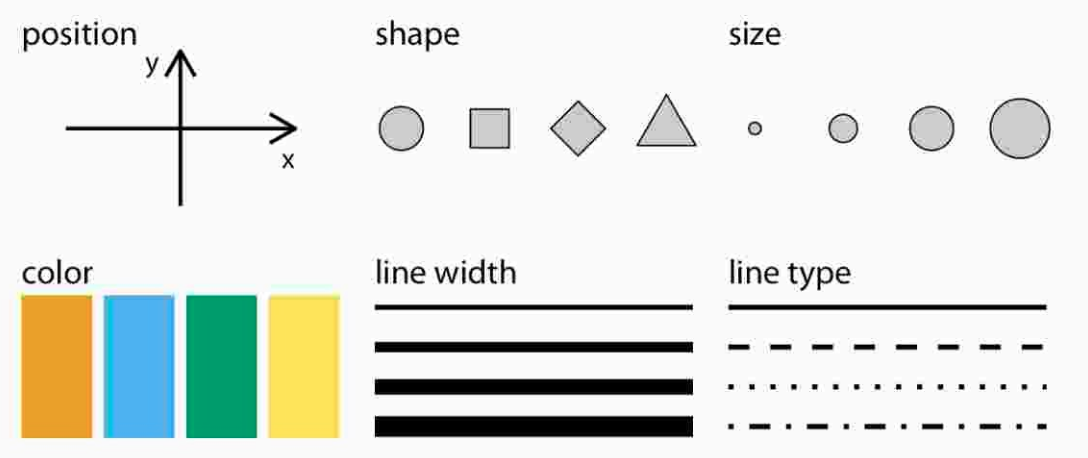
\includegraphics[scale=0.4]{005-3.png}
\end{frame}

\section{How ggplot2 works}
	
		\begin{frame}{ggplot2 to make plots}
		\begin{itemize}
			\item ggplot provides you with a set of	tools to map data 
			\begin{enumerate}
				\item to visual elements on your plot
				\item to specify the kind of plot you want, and 
				\item then subsquently to control the fine details of how it will be displayed.
			\end{enumerate}
		\end{itemize}
	\end{frame}


\begin{frame}{Aesthetic mappings}
\begin{columns}
		\begin{column}{0.5\textwidth}  %%<--- here
		\begin{center}
			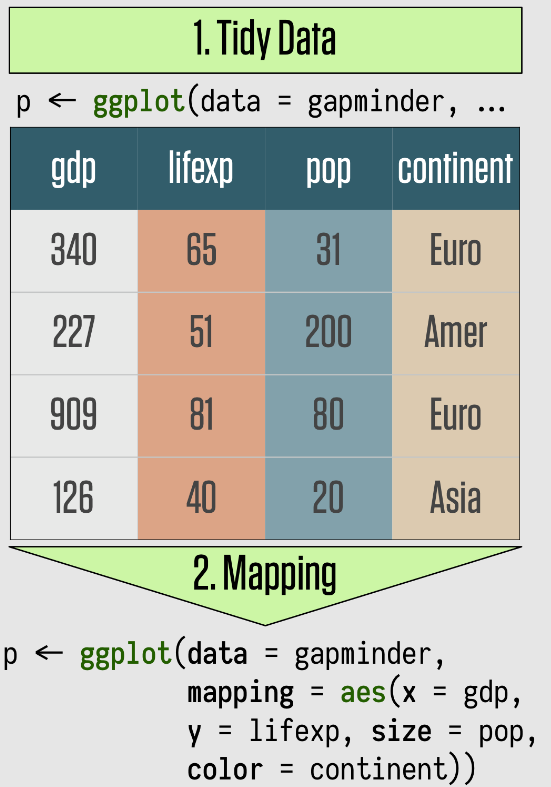
\includegraphics[scale=0.35]{ggplotflow1.png}
		\end{center}
	\end{column}
	\begin{column}{0.5\textwidth}
	\begin{itemize}
	\item The code you write specifies the connections between the variables in your data,
	and the colors, points, and shapes you see on the screen. 
	\item In ggplot, these logical connections between your data and the plot elements are
	called \textit{aesthetic mappings} or just \textit{aesthetics}. 
	\item You begin every plot by telling the \texttt{ggplot()} function what your data is, and then how the
	variables in this data logically map onto the plot's aesthetics. 
\end{itemize}
	\end{column}
\end{columns}
	
\end{frame}




\begin{frame}{Geometry}
	\begin{columns}
		\begin{column}{0.5\textwidth}  %%<--- here
			\begin{center}
				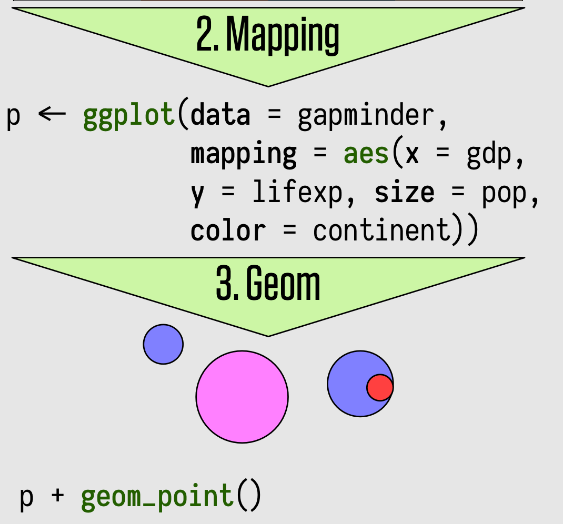
\includegraphics[scale=0.4]{ggplotflow2.png}
			\end{center}
		\end{column}
		\begin{column}{0.5\textwidth}
			\begin{itemize}
				\item Then you take the result and say what general sort of plot you want, such
				as a scatterplot, a boxplot, or a bar chart. In \texttt{ggplot}, the overall
				type of plot is called a \texttt{geom}. 
				\item Each geom has a function that creates it. For example, \texttt{geom\_point()} makes scatterplots, \texttt{geom\_bar()} makes barplots, \texttt{geom\_boxplot()} makes boxplots, and so on. 
				\item You combine these two pieces, the \code{ggplot()} object and the \code{geom}, by literally
				adding them together in an expression, using the ``+'' symbol.
			\end{itemize}
		\end{column}
	\end{columns}
\end{frame}


\begin{frame}{Customization}
	\begin{columns}
		\begin{column}{0.5\textwidth}  %%<--- here
			\begin{center}
				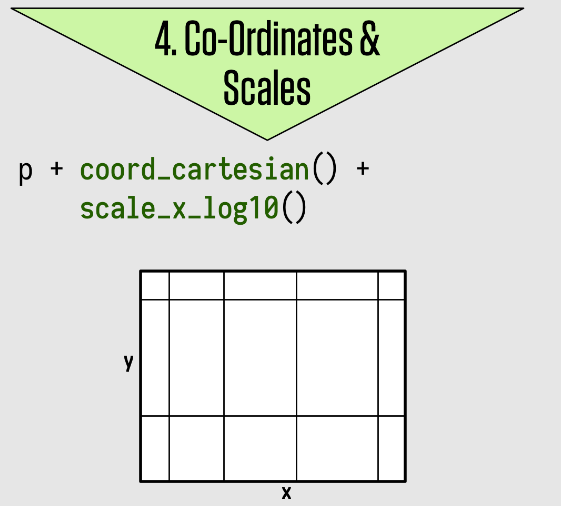
\includegraphics[scale=0.4]{ggplotflow3.png}
			\end{center}
		\end{column}
		\begin{column}{0.5\textwidth}
			\begin{itemize}
				\item At this point, ggplot will have enough information to be able to draw
				a plot for you. ggplot will use a set of defaults that try to be sensible about what gets drawn. 
				\item But more often, you will want to specify exactly what you want, including
				information about the scales, the labels of legends and axes, and
				other guides that help people to read the plot. 
				\item Each component has it own function, you provide arguments to it
				specifying what to do, and you literally add it to the sequence of
				instructions. 
				\item In this way you systematically build your plot piece by
				piece.
			\end{itemize}
		\end{column}
	\end{columns}
\end{frame}



\begin{frame}{Customization}
	\centering
	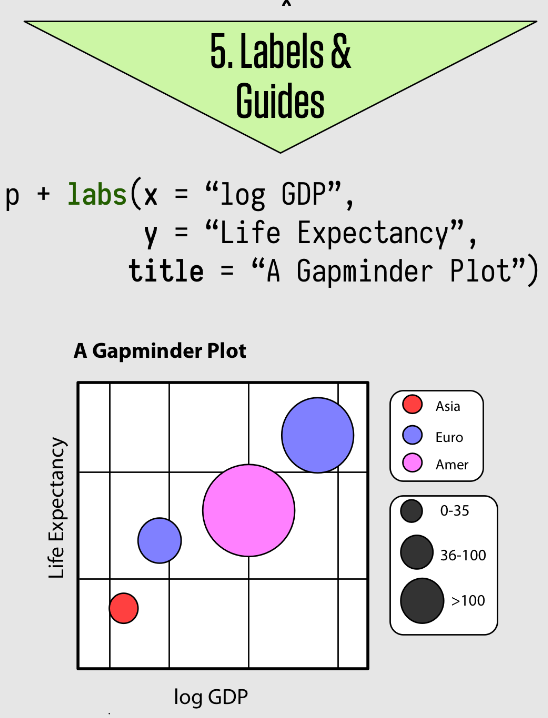
\includegraphics[scale=0.4]{ggplotflow4.png}
\end{frame}


	
\section{Tidy data}

	
\begin{frame}[fragile]{Gapminder dataset in format 1}

\begin{knitrout}\tiny
\definecolor{shadecolor}{rgb}{0.969, 0.969, 0.969}\color{fgcolor}\begin{kframe}
\begin{alltt}
\hlkwd{library}\hlstd{(gapminder)}
\hlstd{gapminder}\hlopt{::}\hlstd{gapminder} \hlopt
  \hlstd{dplyr}\hlopt{::}\hlkwd{select}\hlstd{(country, year, lifeExp)} \hlopt
  \hlstd{tidyr}\hlopt{::}\hlkwd{pivot_wider}\hlstd{(}\hlkwc{names_from} \hlstd{=} \hlstr{"year"}\hlstd{,} \hlkwc{values_from} \hlstd{=} \hlstr{"lifeExp"}\hlstd{)} \hlopt
  \hlstd{dplyr}\hlopt{::}\hlkwd{slice_head}\hlstd{(}\hlkwc{n} \hlstd{=} \hlnum{10}\hlstd{)} \hlopt
  \hlstd{knitr}\hlopt{::}\hlkwd{kable}\hlstd{(}\hlkwc{caption} \hlstd{=} \hlstr{"Life Expectancy data from gapminder dataset for 
  the first 10 countries."}\hlstd{,} \hlkwc{digits} \hlstd{=} \hlnum{0}\hlstd{,} \hlkwc{booktabs}\hlstd{=}\hlnum{TRUE}\hlstd{)}
\end{alltt}
\end{kframe}\begin{table}

\caption{\label{tab:unnamed-chunk-1}Life Expectancy data from gapminder dataset for 
  the first 10 countries.}
\centering
\begin{tabular}[t]{lrrrrrrrrrrrr}
\toprule
country & 1952 & 1957 & 1962 & 1967 & 1972 & 1977 & 1982 & 1987 & 1992 & 1997 & 2002 & 2007\\
\midrule
Afghanistan & 29 & 30 & 32 & 34 & 36 & 38 & 40 & 41 & 42 & 42 & 42 & 44\\
Albania & 55 & 59 & 65 & 66 & 68 & 69 & 70 & 72 & 72 & 73 & 76 & 76\\
Algeria & 43 & 46 & 48 & 51 & 55 & 58 & 61 & 66 & 68 & 69 & 71 & 72\\
Angola & 30 & 32 & 34 & 36 & 38 & 39 & 40 & 40 & 41 & 41 & 41 & 43\\
Argentina & 62 & 64 & 65 & 66 & 67 & 68 & 70 & 71 & 72 & 73 & 74 & 75\\
\addlinespace
Australia & 69 & 70 & 71 & 71 & 72 & 73 & 75 & 76 & 78 & 79 & 80 & 81\\
Austria & 67 & 67 & 70 & 70 & 71 & 72 & 73 & 75 & 76 & 78 & 79 & 80\\
Bahrain & 51 & 54 & 57 & 60 & 63 & 66 & 69 & 71 & 73 & 74 & 75 & 76\\
Bangladesh & 37 & 39 & 41 & 43 & 45 & 47 & 50 & 53 & 56 & 59 & 62 & 64\\
Belgium & 68 & 69 & 70 & 71 & 71 & 73 & 74 & 75 & 76 & 78 & 78 & 79\\
\bottomrule
\end{tabular}
\end{table}

\end{knitrout}

\end{frame}


\begin{frame}[fragile]{Gapminder dataset in format 2}
	
\begin{knitrout}\tiny
\definecolor{shadecolor}{rgb}{0.969, 0.969, 0.969}\color{fgcolor}\begin{kframe}
\begin{alltt}
\hlstd{gapminder}\hlopt{::}\hlstd{gapminder} \hlopt
        \hlstd{dplyr}\hlopt{::}\hlkwd{select}\hlstd{(country, year, lifeExp)} \hlopt
        \hlstd{dplyr}\hlopt{::}\hlkwd{filter}\hlstd{(country} \hlopt \hlkwd{c}\hlstd{(}\hlstr{"Afghanistan"}\hlstd{,}\hlstr{"Albania"}\hlstd{))} \hlopt
        \hlstd{knitr}\hlopt{::}\hlkwd{kable}\hlstd{(}\hlkwc{caption} \hlstd{=} \hlstr{"gapminder dataset for Afghanistan and Albania"}\hlstd{,} \hlkwc{digits} \hlstd{=} \hlnum{0}\hlstd{,} \hlkwc{booktabs}\hlstd{=}\hlnum{TRUE}\hlstd{)}
\end{alltt}
\end{kframe}\begin{table}

\caption{\label{tab:unnamed-chunk-2}gapminder dataset for Afghanistan and Albania}
\centering
\begin{tabular}[t]{lrr}
\toprule
country & year & lifeExp\\
\midrule
Afghanistan & 1952 & 29\\
Afghanistan & 1957 & 30\\
Afghanistan & 1962 & 32\\
Afghanistan & 1967 & 34\\
Afghanistan & 1972 & 36\\
\addlinespace
Afghanistan & 1977 & 38\\
Afghanistan & 1982 & 40\\
Afghanistan & 1987 & 41\\
Afghanistan & 1992 & 42\\
Afghanistan & 1997 & 42\\
\addlinespace
Afghanistan & 2002 & 42\\
Afghanistan & 2007 & 44\\
Albania & 1952 & 55\\
Albania & 1957 & 59\\
Albania & 1962 & 65\\
\addlinespace
Albania & 1967 & 66\\
Albania & 1972 & 68\\
Albania & 1977 & 69\\
Albania & 1982 & 70\\
Albania & 1987 & 72\\
\addlinespace
Albania & 1992 & 72\\
Albania & 1997 & 73\\
Albania & 2002 & 76\\
Albania & 2007 & 76\\
\bottomrule
\end{tabular}
\end{table}

\end{knitrout}
	
\end{frame}


\begin{frame}{Tidy data is usually not compact}
	\begin{itemize}
		\item If you compare the two previous tables, it is clear that a tidy table does not present data in its most compact form. \item In fact, it is usually not how you would choose to present your data if you wanted to just show people the numbers. \item Neither is untidy data “messy” or the “wrong” way to lay out data in some generic sense. 
		\item It's just that, even if its long-form shape makes tables larger, tidy data is much more straightforward to work with when it comes to specifying the mappings that you need to coherently describe plots.
	\end{itemize}
\end{frame}


\section{Mappings link data to things you see}

\begin{frame}{Mappings}
	\begin{itemize}
		\item It’s useful to think of a recipe or template that we start from each time we want to make a plot:
	\end{itemize}
\vspace*{0.5in}
\centering
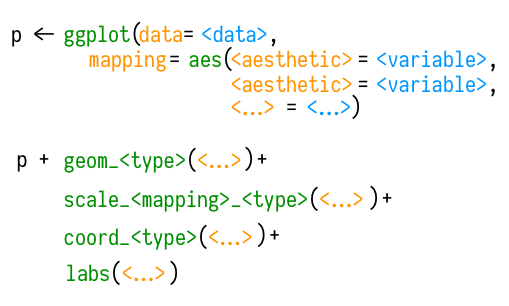
\includegraphics[scale=0.6]{ch-03-ggplot-formula-schematic.png}
\end{frame}



\begin{frame}[fragile]{Gapminder example - the data}
	
	\begin{itemize}
		\item Let’s say we want to plot Life Expectancy against per capita GDP for all country-years in the data. 
		\item  We’ll do this by creating an object that has some of the necessary information in it, and build it up from there. \item First, we must tell the \code{ggplot()} function what data we are using:
	\end{itemize}
	
\begin{knitrout}
\definecolor{shadecolor}{rgb}{0.969, 0.969, 0.969}\color{fgcolor}\begin{kframe}
\begin{alltt}
\hlkwd{library}\hlstd{(ggplot2)}
\hlkwd{library}\hlstd{(cowplot)}
\hlstd{ggplot2}\hlopt{::}\hlkwd{theme_set}\hlstd{(cowplot}\hlopt{::}\hlkwd{theme_cowplot}\hlstd{())}
\hlstd{p} \hlkwb{<-} \hlkwd{ggplot}\hlstd{(}\hlkwc{data} \hlstd{= gapminder)}
\end{alltt}
\end{kframe}
\end{knitrout}
	
\end{frame}

\begin{frame}[fragile]{Gapminder example - mappings}
	
	\begin{itemize}
		\item At this point ggplot knows our data, but not what the mapping. 
		\item That is, we need to tell it which variables in the data should be represented by which visual elements in the plot. \item It also doesn’t know what sort of plot we want. 
		\item In ggplot, mappings are specified using the \code{aes()} function. Like this:
	\end{itemize}
	
\begin{knitrout}
\definecolor{shadecolor}{rgb}{0.969, 0.969, 0.969}\color{fgcolor}\begin{kframe}
\begin{alltt}
\hlstd{p} \hlkwb{<-} \hlkwd{ggplot}\hlstd{(}\hlkwc{data} \hlstd{= gapminder,}
            \hlkwc{mapping} \hlstd{=} \hlkwd{aes}\hlstd{(}\hlkwc{x} \hlstd{= gdpPercap,}
                          \hlkwc{y} \hlstd{= lifeExp))}
\end{alltt}
\end{kframe}
\end{knitrout}
	
\end{frame}



\begin{frame}[fragile]{Gapminder example}
	
	\begin{itemize}
		\item What happens if we just type \code{p} at the console at this point and hit return?
	\end{itemize}

\pause 
	
\begin{knitrout}\tiny
\definecolor{shadecolor}{rgb}{0.969, 0.969, 0.969}\color{fgcolor}\begin{kframe}
\begin{alltt}
\hlstd{p}
\end{alltt}
\end{kframe}

{\centering 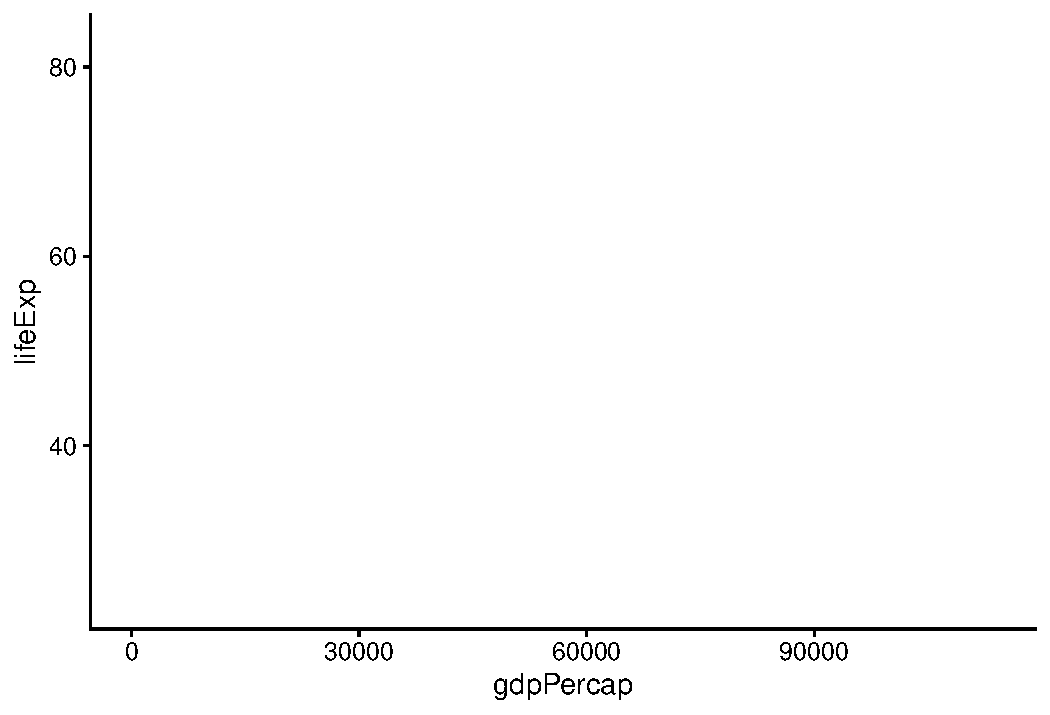
\includegraphics[width=\maxwidth]{figure/unnamed-chunk-5-1} 

}


\end{knitrout}
	
\end{frame}



\begin{frame}[fragile]{Gapminder example - scatterplot}
	
	\begin{itemize}
		\item We need to add a \code{layer} to the plot. This means picking a \code{geom\_} function.
	\end{itemize}
	

\begin{knitrout}\tiny
\definecolor{shadecolor}{rgb}{0.969, 0.969, 0.969}\color{fgcolor}\begin{kframe}
\begin{alltt}
\hlstd{p} \hlopt{+} \hlkwd{geom_point}\hlstd{()}
\end{alltt}
\end{kframe}

{\centering 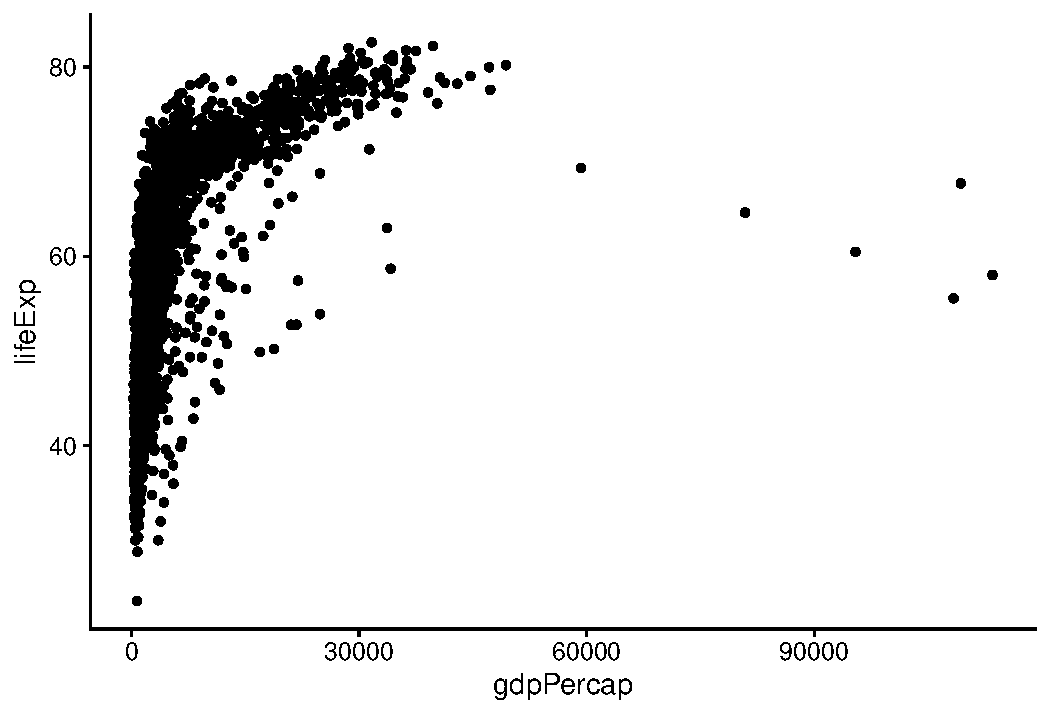
\includegraphics[width=\maxwidth]{figure/unnamed-chunk-6-1} 

}


\end{knitrout}
	
\end{frame}



\section{Build your plots layer by layer}


\begin{frame}{Five steps to build a plot}
	
\begin{enumerate}
	\item Tell the \code{ggplot} function what our data is. The \code{data = …} step.  
\pause	\item  Tell \code{ggplot} \textit{what} relationships we want to see. The \code{mapping = aes(…)} step. For convenience we will put the results of the first two steps in an object called \code{p}.  
\pause	\item  Tell \code{ggplot} \textit{how} we want to see the relationships in our data, i.e. choose a geom.  
\pause	\item  Layer on geoms as needed, by adding them to the \code{p} object one at a time.  
\pause	\item  Use some additional functions to adjust scales, labels, tick marks, titles using the \code{scale\_,} family, \code{labs()} and \code{guides()} functions. We'll learn more about some of these functions shortly.  
\end{enumerate}
\end{frame}


\begin{frame}[fragile]{Add a GAM smoother}
	\begin{columns}
		\begin{column}{0.5\textwidth}  %%<--- here
\begin{knitrout}\tiny
\definecolor{shadecolor}{rgb}{0.969, 0.969, 0.969}\color{fgcolor}\begin{kframe}
\begin{alltt}
\hlstd{p} \hlkwb{<-} \hlkwd{ggplot}\hlstd{(}\hlkwc{data} \hlstd{= gapminder,}
            \hlkwc{mapping} \hlstd{=} \hlkwd{aes}\hlstd{(}\hlkwc{x} \hlstd{= gdpPercap,}
                          \hlkwc{y}\hlstd{=lifeExp))}
\hlstd{p} \hlopt{+} \hlkwd{geom_smooth}\hlstd{()}
\end{alltt}


{\ttfamily\noindent\itshape\color{messagecolor}{\#\# `geom\_smooth()` using method = 'gam' and formula 'y \textasciitilde{} s(x, bs = "{}cs"{})'}}\end{kframe}

{\centering 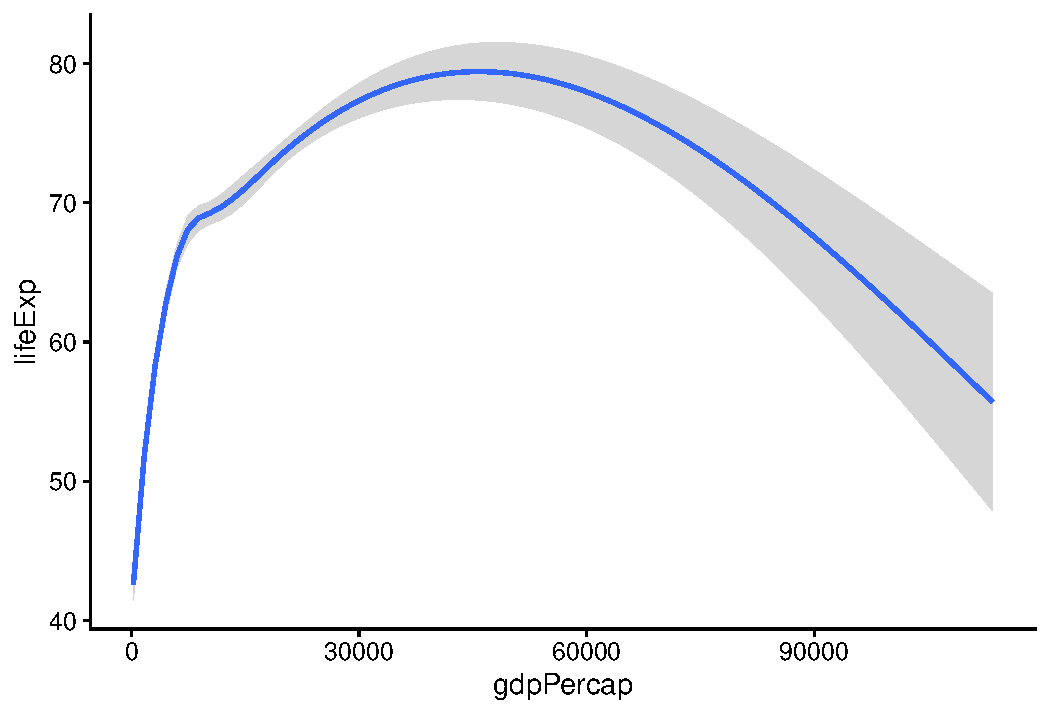
\includegraphics[width=\maxwidth]{figure/unnamed-chunk-7-1} 

}


\end{knitrout}
		\end{column}
		\begin{column}{0.5\textwidth}
			\begin{itemize}
					\item The coordinate system used in plots is most often cartesian, i.e., a plane defined by an x axis and a y axis. This is	what ggplot assumes, unless you tell it otherwise. \pause 
				\item Usually in R, functions cannot simply be added to objects. Rather, they take objects as inputs and produce objects as outputs.
				\item But the objects created by \code{ggplot()} are special. This makes it easier to assemble plots one piece at a time, and to inspect how they look at every step. 
			\end{itemize}
		\end{column}
	\end{columns}
\end{frame}







\begin{frame}[fragile]{Add a linear smoother with data points}
	\begin{columns}
		\begin{column}{0.5\textwidth}  %%<--- here
\begin{knitrout}\tiny
\definecolor{shadecolor}{rgb}{0.969, 0.969, 0.969}\color{fgcolor}\begin{kframe}
\begin{alltt}
\hlstd{p} \hlkwb{<-} \hlkwd{ggplot}\hlstd{(}\hlkwc{data} \hlstd{= gapminder,}
\hlkwc{mapping} \hlstd{=} \hlkwd{aes}\hlstd{(}\hlkwc{x} \hlstd{= gdpPercap,}
\hlkwc{y}\hlstd{=lifeExp))}
\hlstd{p} \hlopt{+} \hlkwd{geom_point}\hlstd{()} \hlopt{+} \hlkwd{geom_smooth}\hlstd{(}\hlkwc{method} \hlstd{=} \hlstr{"lm"}\hlstd{)}
\end{alltt}


{\ttfamily\noindent\itshape\color{messagecolor}{\#\# `geom\_smooth()` using formula 'y \textasciitilde{} x'}}\end{kframe}

{\centering 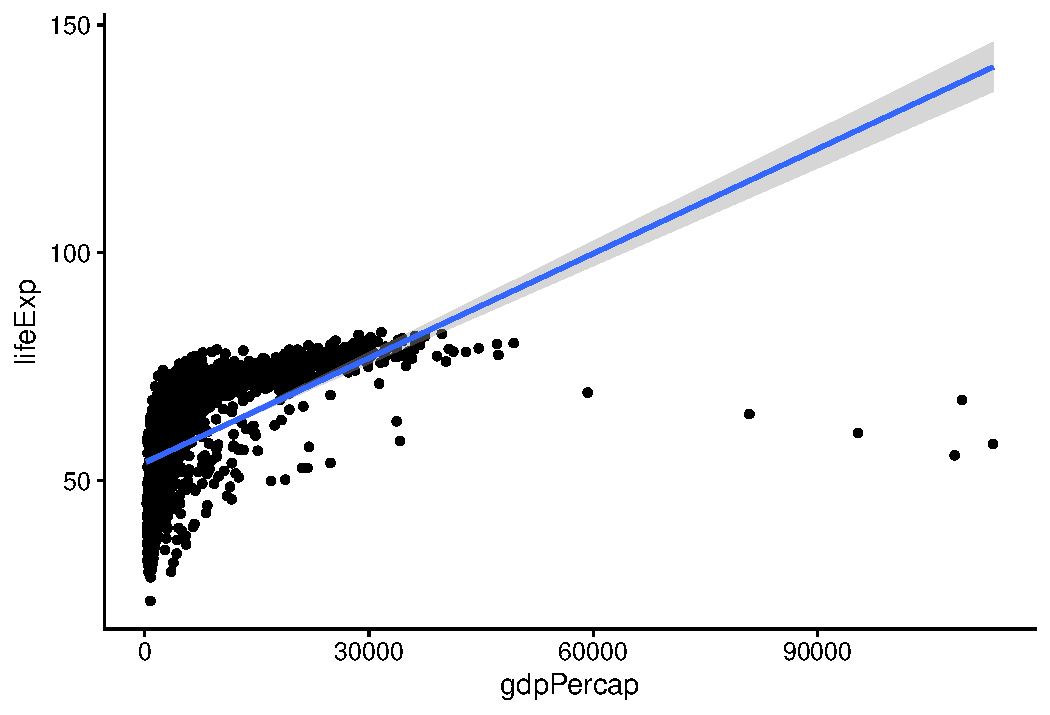
\includegraphics[width=\maxwidth]{figure/unnamed-chunk-8-1} 

}


\end{knitrout}
		\end{column}\pause 
		\begin{column}{0.5\textwidth}
			\begin{itemize}
				\item We did not have to tell \code{geom\_point()} or \code{geom\_smooth()}
				where their data was coming from, or what mappings they should use.
\pause	\item 			They \textit{inherit} this information from the original \code{p} object. 
	\item As we'll see later, it’s possible to give geoms separate instructions that they
				will follow instead. But in the absence of any other information, the
				geoms will look for the instructions it needs in the \code{ggplot()}
				function, or the object created by it.
			\end{itemize}
		\end{column}
	\end{columns}
\end{frame}





\begin{frame}[fragile]{Change scales}
	\begin{columns}
		\begin{column}{0.5\textwidth}  %%<--- here
\begin{knitrout}\tiny
\definecolor{shadecolor}{rgb}{0.969, 0.969, 0.969}\color{fgcolor}\begin{kframe}
\begin{alltt}
\hlstd{p} \hlkwb{<-} \hlkwd{ggplot}\hlstd{(}\hlkwc{data} \hlstd{= gapminder,}
        \hlkwc{mapping} \hlstd{=} \hlkwd{aes}\hlstd{(}\hlkwc{x} \hlstd{= gdpPercap,}
                \hlkwc{y}\hlstd{=lifeExp))}
\hlstd{p} \hlopt{+} \hlkwd{geom_point}\hlstd{()} \hlopt{+}
        \hlkwd{geom_smooth}\hlstd{(}\hlkwc{method} \hlstd{=} \hlstr{"gam"}\hlstd{)} \hlopt{+}
        \hlkwd{scale_x_log10}\hlstd{()}
\end{alltt}


{\ttfamily\noindent\itshape\color{messagecolor}{\#\# `geom\_smooth()` using formula 'y \textasciitilde{} s(x, bs = "{}cs"{})'}}\end{kframe}

{\centering 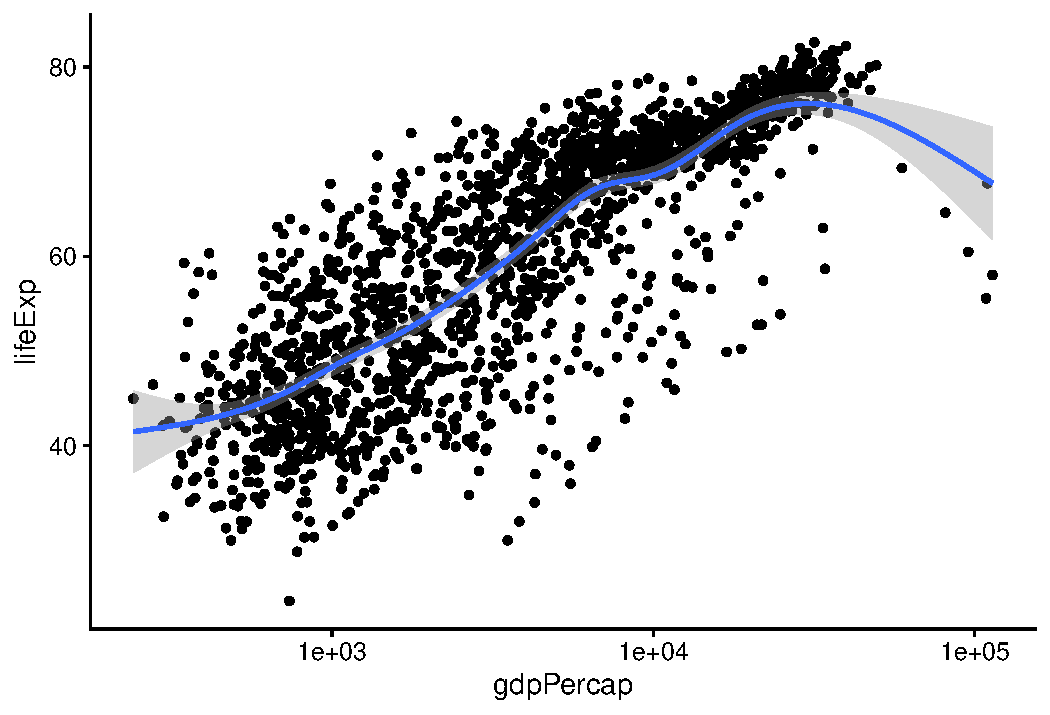
\includegraphics[width=\maxwidth]{figure/unnamed-chunk-9-1} 

}


\end{knitrout}
		\end{column}\pause 
		\begin{column}{0.5\textwidth}
			\begin{itemize}
				\item The data is quite bunched up against the left side. 
				\item Gross Domestic Product per capita is not normally distributed across our country years. 
				\item The x-axis scale would probably look better if it were transformed from a linear scale to a log scale. For this we can use a function called \code{scale\_x\_log10()}. 
				\item As you might expect this function scales the x-axis of a plot to a log 10 basis. 
			\end{itemize}
		\end{column}
	\end{columns}
\end{frame}




\begin{frame}[fragile]{Formatting labels with the \texttt{scales} package}
\begin{knitrout}\tiny
\definecolor{shadecolor}{rgb}{0.969, 0.969, 0.969}\color{fgcolor}\begin{kframe}
\begin{alltt}
\hlkwd{library}\hlstd{(scales)}
\hlstd{p} \hlkwb{<-} \hlkwd{ggplot}\hlstd{(}\hlkwc{data} \hlstd{= gapminder,} \hlkwc{mapping} \hlstd{=} \hlkwd{aes}\hlstd{(}\hlkwc{x} \hlstd{= gdpPercap,} \hlkwc{y}\hlstd{=lifeExp))}
\hlstd{p} \hlopt{+} \hlkwd{geom_point}\hlstd{()} \hlopt{+}
        \hlkwd{geom_smooth}\hlstd{(}\hlkwc{method} \hlstd{=} \hlstr{"gam"}\hlstd{)} \hlopt{+}
        \hlkwd{scale_x_log10}\hlstd{(}\hlkwc{labels} \hlstd{= scales}\hlopt{::}\hlstd{dollar)}
\end{alltt}
\end{kframe}

{\centering 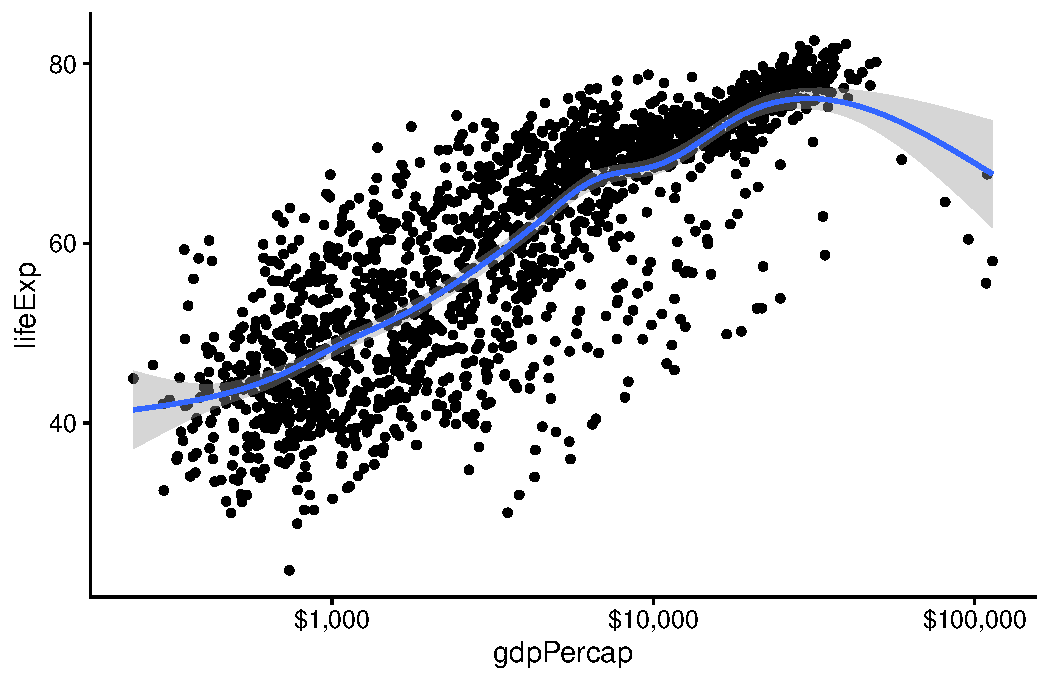
\includegraphics[width=\maxwidth]{figure/unnamed-chunk-10-1} 

}


\end{knitrout}

\end{frame}



\section{Mapping aesthetics vs setting them}


\begin{frame}[fragile]{Color aesthetic}
\begin{itemize}
	\item An \textit{aesthetic mapping} specifies that a variable will be expressed by one of the available visual elements, such as size, or color, or shape, and so on. As we've seen, we map variables to aesthetics like this: 
\begin{knitrout}
\definecolor{shadecolor}{rgb}{0.969, 0.969, 0.969}\color{fgcolor}\begin{kframe}
\begin{alltt}
\hlstd{p} \hlkwb{<-}  \hlkwd{ggplot}\hlstd{(}\hlkwc{data} \hlstd{= gapminder,}
                \hlkwc{mapping} \hlstd{=} \hlkwd{aes}\hlstd{(}\hlkwc{x} \hlstd{= gdpPercap,}
                                \hlkwc{y} \hlstd{= lifeExp,}
                                \hlkwc{color} \hlstd{= continent))}
\end{alltt}
\end{kframe}
\end{knitrout}
	\pause
	\item This code does \textit{not} give a direct instruction like ``color the points purple''. \pause
	\item Instead it says, ``the variable continent will map onto the color aesthetic''. 
\end{itemize}
	
\end{frame}


\begin{frame}[fragile]{Misunderstanding of an aesthetic}
	\begin{itemize}
		\item If we want to turn all the points in the figure purple, we do \textit{not} do it through the mapping function. Look at what happens when we try:
\begin{knitrout}\tiny
\definecolor{shadecolor}{rgb}{0.969, 0.969, 0.969}\color{fgcolor}\begin{kframe}
\begin{alltt}
\hlstd{p} \hlkwb{<-} \hlkwd{ggplot}\hlstd{(}\hlkwc{data} \hlstd{= gapminder,}
                        \hlkwc{mapping} \hlstd{=} \hlkwd{aes}\hlstd{(}\hlkwc{x} \hlstd{= gdpPercap,}
                        \hlkwc{y} \hlstd{= lifeExp,}
                        \hlkwc{color} \hlstd{=} \hlstr{"purple"}\hlstd{))}
\hlstd{p} \hlopt{+} \hlkwd{geom_point}\hlstd{()} \hlopt{+}
        \hlkwd{geom_smooth}\hlstd{(}\hlkwc{method} \hlstd{=} \hlstr{"loess"}\hlstd{)} \hlopt{+}
        \hlkwd{scale_x_log10}\hlstd{()}
\end{alltt}
\end{kframe}

{\centering 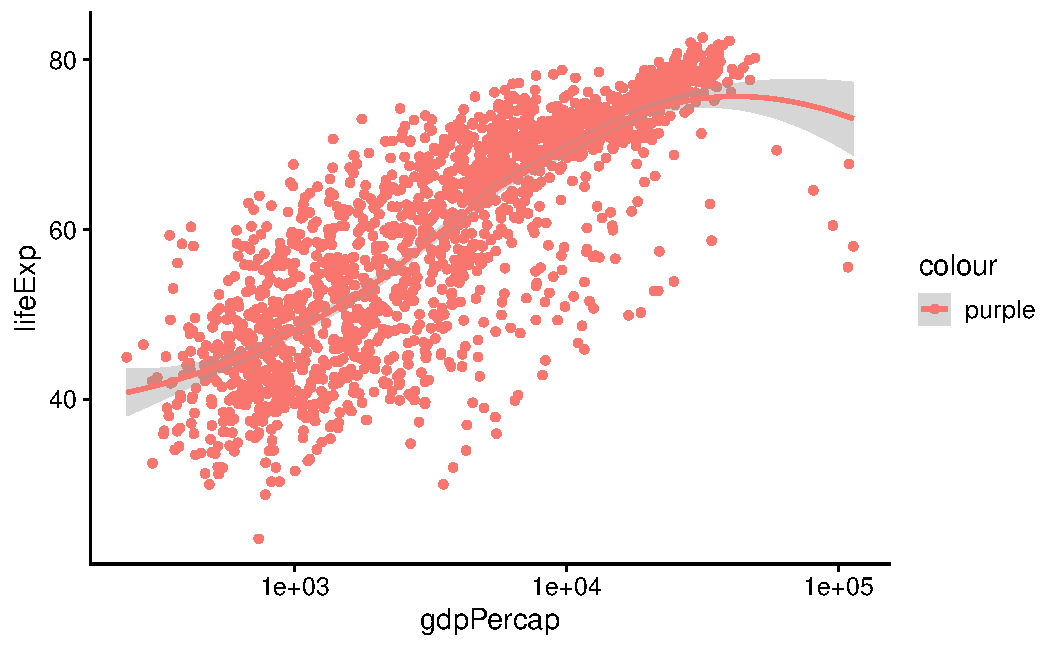
\includegraphics[width=\maxwidth]{figure/unnamed-chunk-12-1} 

}


\end{knitrout}
	\end{itemize}
	
\end{frame}




\begin{frame}[fragile]{The correct way of specifying point colors}
\begin{knitrout}\tiny
\definecolor{shadecolor}{rgb}{0.969, 0.969, 0.969}\color{fgcolor}\begin{kframe}
\begin{alltt}
\hlstd{p} \hlkwb{<-} \hlkwd{ggplot}\hlstd{(}\hlkwc{data} \hlstd{= gapminder,}
                        \hlkwc{mapping} \hlstd{=} \hlkwd{aes}\hlstd{(}\hlkwc{x} \hlstd{= gdpPercap,}
                                        \hlkwc{y} \hlstd{= lifeExp))}
\hlstd{p} \hlopt{+} \hlkwd{geom_point}\hlstd{(}\hlkwc{color} \hlstd{=} \hlstr{"purple"}\hlstd{)} \hlopt{+}
        \hlkwd{geom_smooth}\hlstd{(}\hlkwc{method} \hlstd{=} \hlstr{"loess"}\hlstd{)} \hlopt{+}
        \hlkwd{scale_x_log10}\hlstd{()}
\end{alltt}
\end{kframe}

{\centering 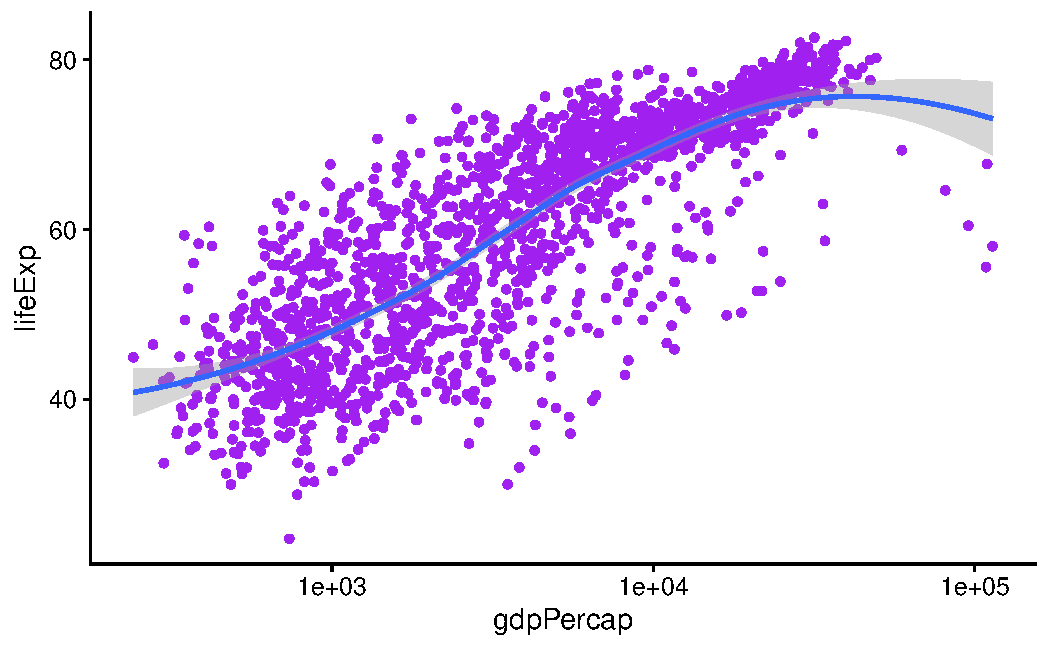
\includegraphics[width=\maxwidth]{figure/unnamed-chunk-13-1} 

}


\end{knitrout}
\end{frame}



\begin{frame}[fragile]{\code{geom\_} functions can take many other arguments that will affect how the plot looks}
\begin{knitrout}\tiny
\definecolor{shadecolor}{rgb}{0.969, 0.969, 0.969}\color{fgcolor}\begin{kframe}
\begin{alltt}
\hlstd{p} \hlkwb{<-} \hlkwd{ggplot}\hlstd{(}\hlkwc{data} \hlstd{= gapminder,}
                \hlkwc{mapping} \hlstd{=} \hlkwd{aes}\hlstd{(}\hlkwc{x} \hlstd{= gdpPercap,}
                                        \hlkwc{y} \hlstd{= lifeExp))}
\hlstd{p} \hlopt{+} \hlkwd{geom_point}\hlstd{(}\hlkwc{alpha} \hlstd{=} \hlnum{0.3}\hlstd{)} \hlopt{+}
\hlkwd{geom_smooth}\hlstd{(}\hlkwc{color} \hlstd{=} \hlstr{"orange"}\hlstd{,} \hlkwc{se} \hlstd{=} \hlnum{FALSE}\hlstd{,} \hlkwc{size} \hlstd{=} \hlnum{8}\hlstd{,} \hlkwc{method} \hlstd{=} \hlstr{"lm"}\hlstd{)} \hlopt{+}
\hlkwd{scale_x_log10}\hlstd{()}
\end{alltt}
\end{kframe}

{\centering 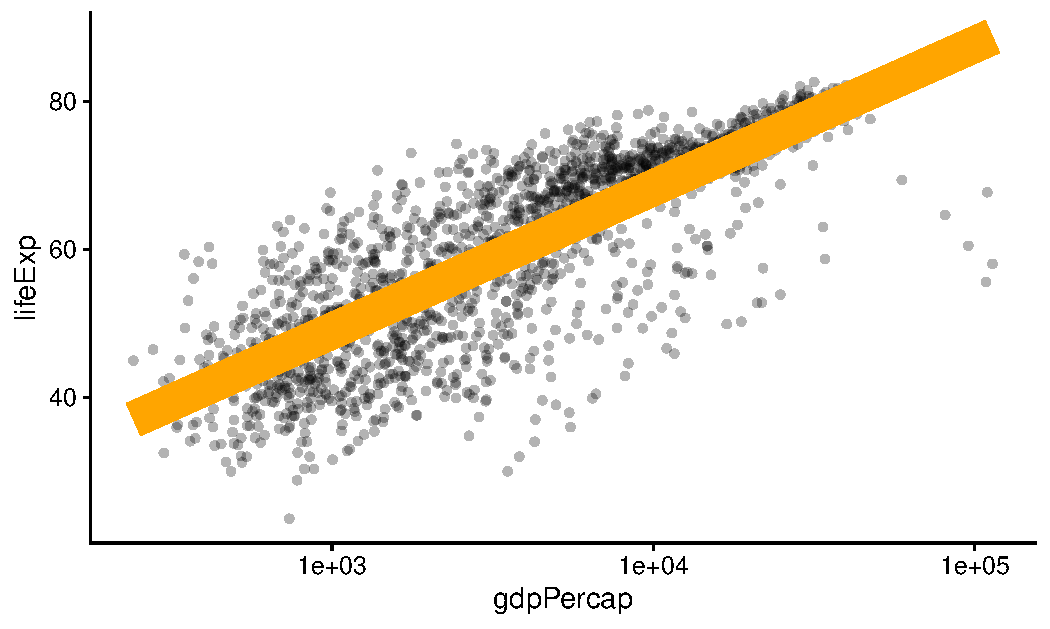
\includegraphics[width=\maxwidth]{figure/unnamed-chunk-14-1} 

}


\end{knitrout}
\end{frame}



\begin{frame}[fragile]{Add lables and change themes}
\begin{knitrout}\tiny
\definecolor{shadecolor}{rgb}{0.969, 0.969, 0.969}\color{fgcolor}\begin{kframe}
\begin{alltt}
\hlstd{p} \hlkwb{<-} \hlkwd{ggplot}\hlstd{(}\hlkwc{data} \hlstd{= gapminder,} \hlkwc{mapping} \hlstd{=} \hlkwd{aes}\hlstd{(}\hlkwc{x} \hlstd{= gdpPercap,} \hlkwc{y}\hlstd{=lifeExp))}
\hlstd{p} \hlopt{+} \hlkwd{geom_point}\hlstd{(}\hlkwc{alpha} \hlstd{=} \hlnum{0.3}\hlstd{)} \hlopt{+} \hlkwd{geom_smooth}\hlstd{(}\hlkwc{method} \hlstd{=} \hlstr{"gam"}\hlstd{)} \hlopt{+}
    \hlkwd{scale_x_log10}\hlstd{(}\hlkwc{labels} \hlstd{= scales}\hlopt{::}\hlstd{dollar)} \hlopt{+}
    \hlstd{ggthemes}\hlopt{::}\hlkwd{theme_stata}\hlstd{()} \hlopt{+}
    \hlkwd{labs}\hlstd{(}\hlkwc{x} \hlstd{=} \hlstr{"GDP Per Capita"}\hlstd{,} \hlkwc{y} \hlstd{=} \hlstr{"Life Expectancy in Years"}\hlstd{,}
        \hlkwc{title} \hlstd{=} \hlstr{"Economic Growth and Life Expectancy"}\hlstd{,}
        \hlkwc{subtitle} \hlstd{=} \hlstr{"Data points are country-years"}\hlstd{,}
        \hlkwc{caption} \hlstd{=} \hlstr{"Source: Gapminder."}\hlstd{)}
\end{alltt}
\end{kframe}

{\centering 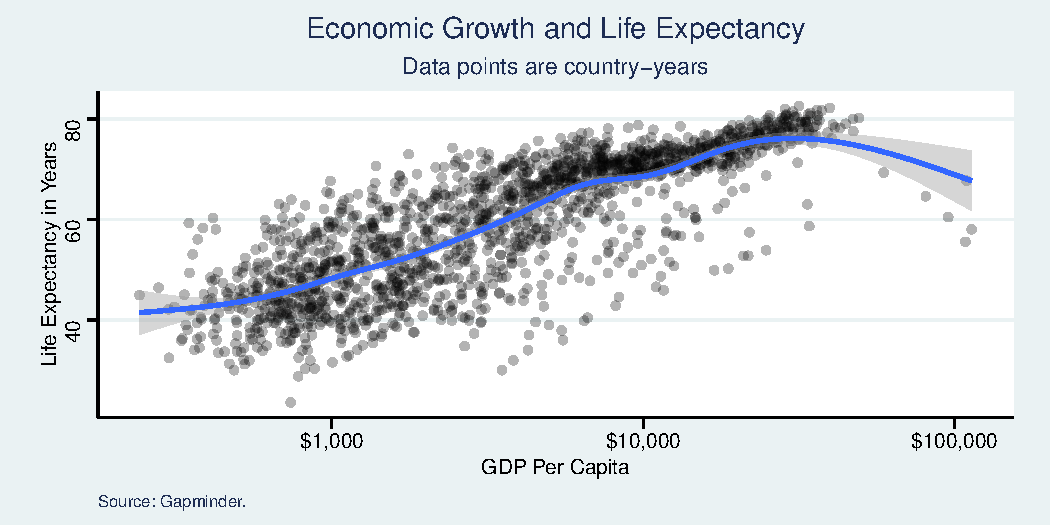
\includegraphics[width=\maxwidth]{figure/unnamed-chunk-15-1} 

}


\end{knitrout}
\end{frame}




\begin{frame}[fragile]{Smooth lines for each continent}
	\begin{itemize}
		\item Along with \code{x} and \code{y}, the \code{color} aesthetic mapping is set in the call to \code{ggplot} that we used to create the \code{p} object
\begin{knitrout}\tiny
\definecolor{shadecolor}{rgb}{0.969, 0.969, 0.969}\color{fgcolor}\begin{kframe}
\begin{alltt}
\hlstd{p} \hlkwb{<-} \hlkwd{ggplot}\hlstd{(}\hlkwc{data} \hlstd{= gapminder,}
            \hlkwc{mapping} \hlstd{=} \hlkwd{aes}\hlstd{(}\hlkwc{x} \hlstd{= gdpPercap,}
            \hlkwc{y} \hlstd{= lifeExp,}
            \hlkwc{color} \hlstd{= continent))}
\hlstd{p} \hlopt{+} \hlkwd{geom_point}\hlstd{()} \hlopt{+}
        \hlkwd{geom_smooth}\hlstd{(}\hlkwc{method} \hlstd{=} \hlstr{"loess"}\hlstd{)} \hlopt{+}
        \hlkwd{scale_x_log10}\hlstd{()}
\end{alltt}
\end{kframe}

{\centering 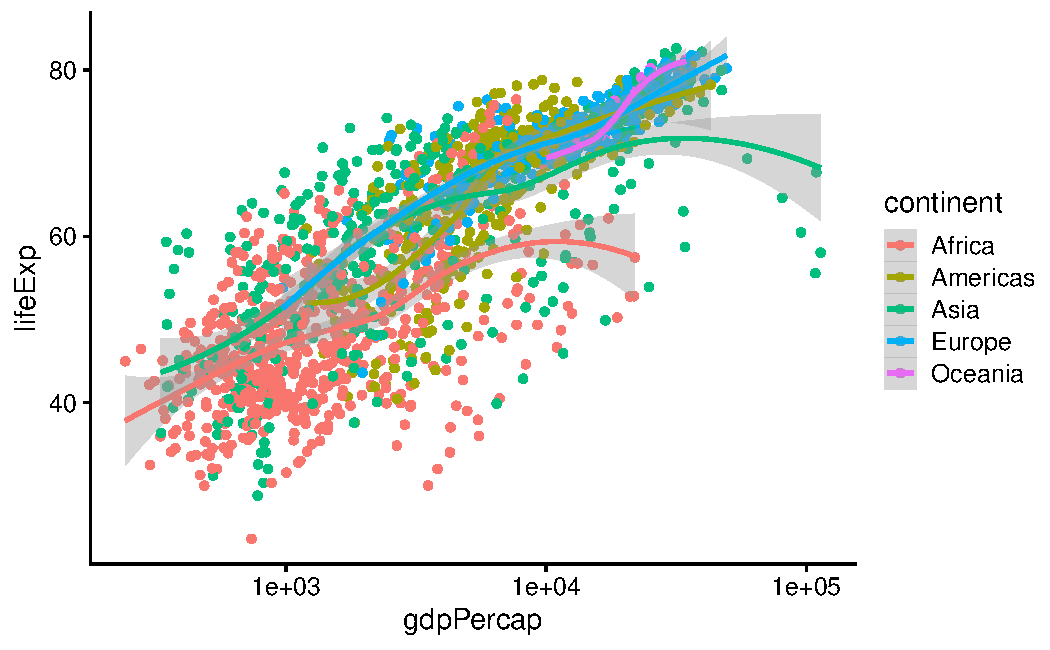
\includegraphics[width=\maxwidth]{figure/unnamed-chunk-16-1} 

}


\end{knitrout}
	\end{itemize}
	
\end{frame}


\begin{frame}[fragile]{Standard errors bars with matching color}
\begin{knitrout}\tiny
\definecolor{shadecolor}{rgb}{0.969, 0.969, 0.969}\color{fgcolor}\begin{kframe}
\begin{alltt}
\hlstd{p} \hlkwb{<-} \hlkwd{ggplot}\hlstd{(}\hlkwc{data} \hlstd{= gapminder,}
                \hlkwc{mapping} \hlstd{=} \hlkwd{aes}\hlstd{(}\hlkwc{x} \hlstd{= gdpPercap,}
                \hlkwc{y} \hlstd{= lifeExp,}
                \hlkwc{color} \hlstd{= continent,}
                \hlkwc{fill} \hlstd{= continent))}
\hlstd{p} \hlopt{+} \hlkwd{geom_point}\hlstd{()} \hlopt{+}
\hlkwd{geom_smooth}\hlstd{(}\hlkwc{method} \hlstd{=} \hlstr{"loess"}\hlstd{)} \hlopt{+}
\hlkwd{scale_x_log10}\hlstd{()}
\end{alltt}
\end{kframe}

{\centering 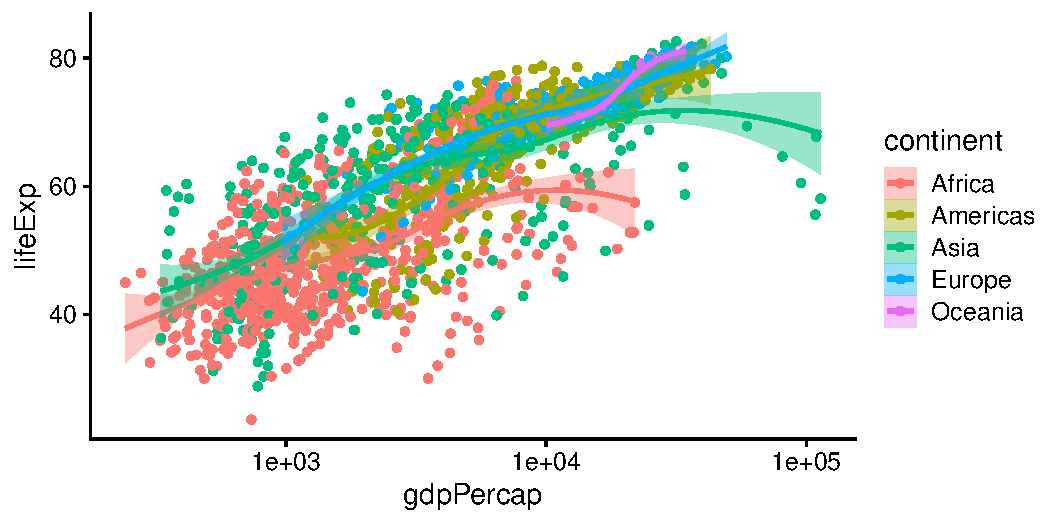
\includegraphics[width=\maxwidth]{figure/unnamed-chunk-17-1} 

}


\end{knitrout}
\end{frame}






\section{Aesthetics can be mapped per geom}

\begin{frame}[fragile]{Specify different mapping for each geom}
	\small
	\begin{itemize}
		\item Perhaps five separate smoothers is too many, and we just want one line. But we still would like to have the points color-coded by continent. By default, geoms inherit their mappings from the \code{ggplot()} function \pause
		\item We can change this by mapping the aesthetics we want only the \code{geom\_} functions that we want them to apply to.\pause
\begin{knitrout}\tiny
\definecolor{shadecolor}{rgb}{0.969, 0.969, 0.969}\color{fgcolor}\begin{kframe}
\begin{alltt}
\hlstd{p} \hlkwb{<-} \hlkwd{ggplot}\hlstd{(}\hlkwc{data} \hlstd{= gapminder,} \hlkwc{mapping} \hlstd{=} \hlkwd{aes}\hlstd{(}\hlkwc{x} \hlstd{= gdpPercap,} \hlkwc{y} \hlstd{= lifeExp))}
\hlstd{p} \hlopt{+} \hlkwd{geom_point}\hlstd{(}\hlkwc{mapping} \hlstd{=} \hlkwd{aes}\hlstd{(}\hlkwc{color} \hlstd{= continent))} \hlopt{+}
        \hlkwd{geom_smooth}\hlstd{(}\hlkwc{method} \hlstd{=} \hlstr{"loess"}\hlstd{)} \hlopt{+}
        \hlkwd{scale_x_log10}\hlstd{()}
\end{alltt}
\end{kframe}

{\centering 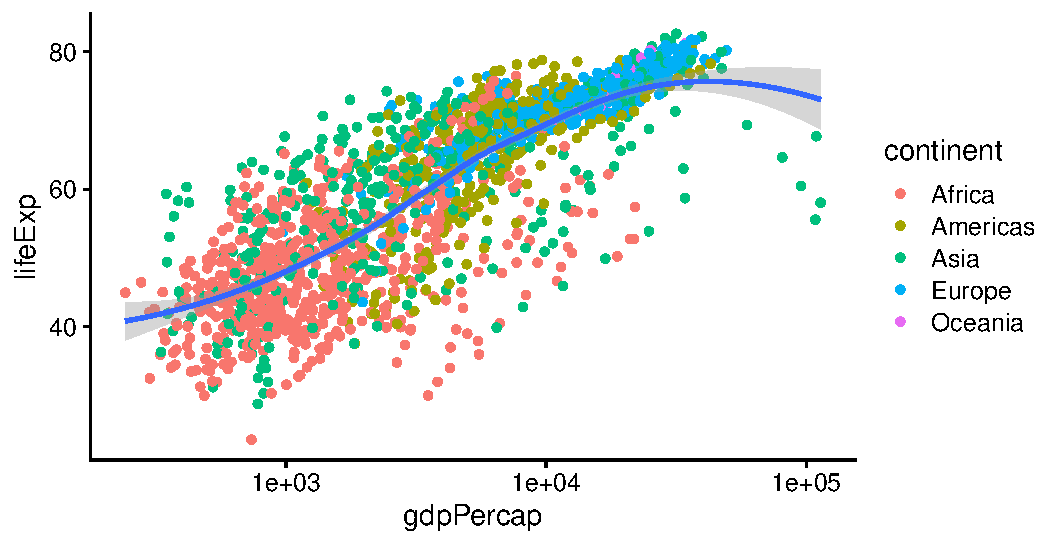
\includegraphics[width=\maxwidth]{figure/unnamed-chunk-18-1} 

}


\end{knitrout}
\end{itemize}
	
\end{frame}


\begin{frame}{A closer look at the legends}
	\centering
	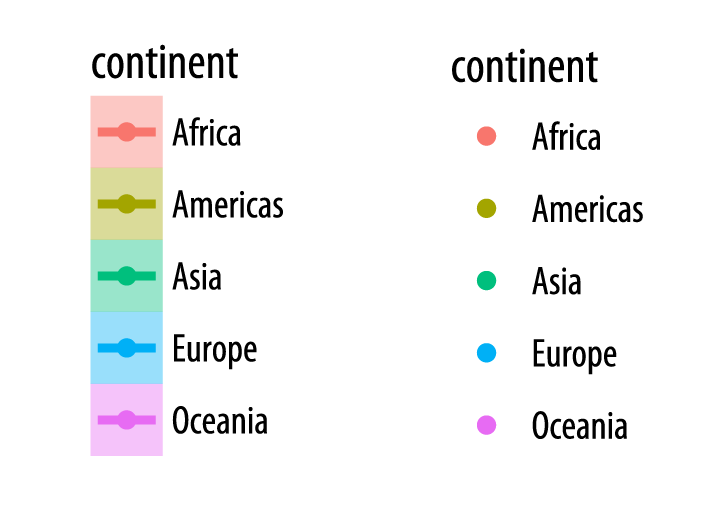
\includegraphics[scale=1]{ch-03-legends-combined.png}
\end{frame}


\begin{frame}[fragile]{Mapping a continuous variable to color}
\begin{knitrout}\tiny
\definecolor{shadecolor}{rgb}{0.969, 0.969, 0.969}\color{fgcolor}\begin{kframe}
\begin{alltt}
\hlstd{p} \hlkwb{<-} \hlkwd{ggplot}\hlstd{(}\hlkwc{data} \hlstd{= gapminder,}
            \hlkwc{mapping} \hlstd{=} \hlkwd{aes}\hlstd{(}\hlkwc{x} \hlstd{= gdpPercap,}
                          \hlkwc{y} \hlstd{= lifeExp))}
\hlstd{p} \hlopt{+} \hlkwd{geom_point}\hlstd{(}\hlkwc{mapping} \hlstd{=} \hlkwd{aes}\hlstd{(}\hlkwc{color} \hlstd{=} \hlkwd{log}\hlstd{(pop)))} \hlopt{+}
                 \hlkwd{scale_x_log10}\hlstd{()}
\end{alltt}
\end{kframe}

{\centering 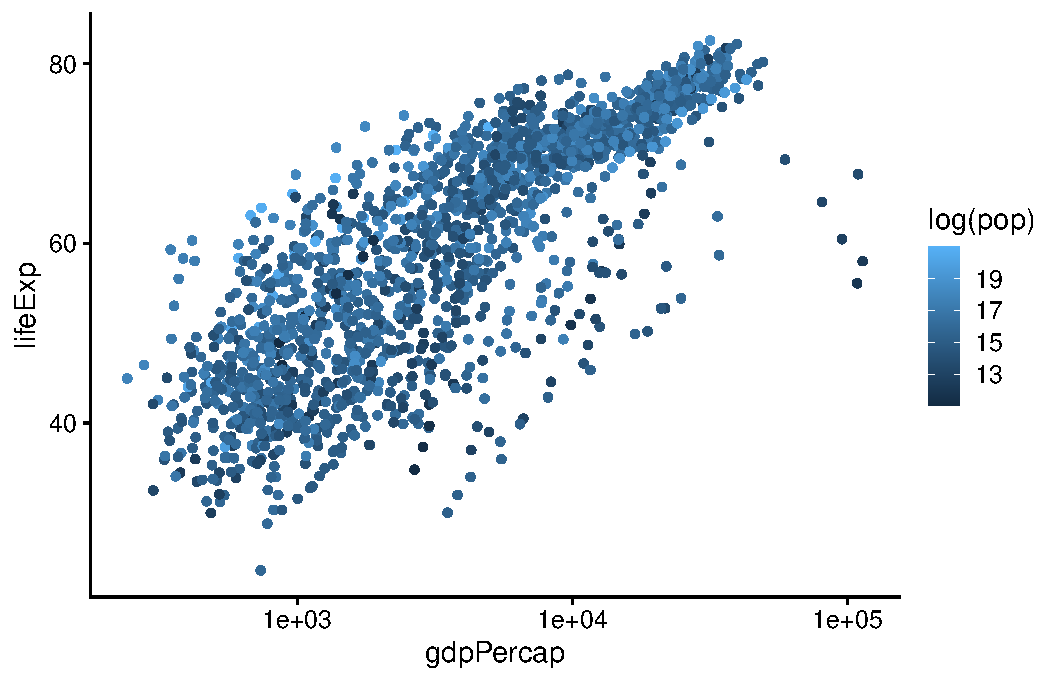
\includegraphics[width=\maxwidth]{figure/unnamed-chunk-19-1} 

}


\end{knitrout}

	
\end{frame}


	\begin{frame}[fragile]{Session Info}
	\tiny
	
\begin{knitrout}\tiny
\definecolor{shadecolor}{rgb}{0.969, 0.969, 0.969}\color{fgcolor}\begin{kframe}
\begin{verbatim}
R version 4.0.2 (2020-06-22)
Platform: x86_64-pc-linux-gnu (64-bit)
Running under: Pop!_OS 20.10

Matrix products: default
BLAS:   /usr/lib/x86_64-linux-gnu/openblas-pthread/libblas.so.3
LAPACK: /usr/lib/x86_64-linux-gnu/openblas-pthread/libopenblasp-r0.3.10.so

attached base packages:
[1] tools     stats     graphics  grDevices utils     datasets  methods  
[8] base     

other attached packages:
 [1] scales_1.1.1     cowplot_1.1.0    DT_0.16          kableExtra_1.2.1
 [5] socviz_1.2       gapminder_0.3.0  here_0.1         NCStats_0.4.7   
 [9] FSA_0.8.30       forcats_0.5.1    stringr_1.4.0    dplyr_1.0.7     
[13] purrr_0.3.4      readr_1.4.0      tidyr_1.1.3      tibble_3.1.3    
[17] ggplot2_3.3.5    tidyverse_1.3.0  knitr_1.33      

loaded via a namespace (and not attached):
 [1] nlme_3.1-149       fs_1.5.0           lubridate_1.7.9    webshot_0.5.2     
 [5] httr_1.4.2         rprojroot_2.0.2    backports_1.2.1    utf8_1.2.2        
 [9] R6_2.5.1           mgcv_1.8-33        DBI_1.1.1          colorspace_2.0-2  
[13] withr_2.4.2        tidyselect_1.1.1   gridExtra_2.3      leaflet_2.0.3     
[17] curl_4.3.2         compiler_4.0.2     cli_3.0.1          rvest_1.0.0       
[21] pacman_0.5.1       xml2_1.3.2         ggdendro_0.1.22    labeling_0.4.2    
[25] mosaicCore_0.8.0   digest_0.6.27      ggformula_0.9.4    foreign_0.8-80    
[29] rmarkdown_2.9.7    rio_0.5.16         pkgconfig_2.0.3    htmltools_0.5.2   
[33] highr_0.9          dbplyr_1.4.4       fastmap_1.1.0      ggthemes_4.2.4    
[37] htmlwidgets_1.5.3  rlang_0.4.11       readxl_1.3.1       rstudioapi_0.13   
[41] farver_2.1.0       generics_0.1.0     jsonlite_1.7.2     crosstalk_1.1.1   
[45] zip_2.2.0          car_3.0-9          magrittr_2.0.1     mosaicData_0.20.1 
[49] Matrix_1.2-18      Rcpp_1.0.7         munsell_0.5.0      fansi_0.5.0       
[53] abind_1.4-5        lifecycle_1.0.0    stringi_1.7.3      carData_3.0-4     
[57] MASS_7.3-53        plyr_1.8.6         ggstance_0.3.4     grid_4.0.2        
[61] blob_1.2.1         ggrepel_0.8.2      crayon_1.4.1       lattice_0.20-41   
[65] haven_2.3.1        splines_4.0.2      hms_1.0.0          pillar_1.6.2      
[69] reprex_0.3.0       glue_1.4.2         evaluate_0.14      data.table_1.14.0 
[73] modelr_0.1.8       vctrs_0.3.8        tweenr_1.0.1       cellranger_1.1.0  
[77] gtable_0.3.0       polyclip_1.10-0    assertthat_0.2.1   TeachingDemos_2.12
[81] xfun_0.25          ggforce_0.3.2      openxlsx_4.1.5     broom_0.7.2       
[85] viridisLite_0.4.0  mosaic_1.7.0       ellipsis_0.3.2    
\end{verbatim}
\end{kframe}
\end{knitrout}
	
\end{frame}

\end{document}



